\documentclass{article}
\usepackage[utf8]{inputenc}
\usepackage{amssymb}
\usepackage[russian]{babel}
\usepackage{amsmath}
\usepackage{graphicx}
\begin{document}

Я всегда тяготел к экзотическим животным — змеям, черепахам. А жаб любил с самого детства. Ведь у них такой «улыбчивый» разрез рта, замечательные глаза с серебристой или золотистой крапинкой — куда там человеческим! Очень миролюбивы и неторопливы — незаменимые качества для хорошего соседа.\newline

\[((\sin(\cos(\sinh((x^{4}))))^{3})-\frac{(x-1)}{(x+2)})\]
\[((\sin(\cos(\sinh((x^{4}))))^{3})-\frac{(x-1)}{(x+2)})\]
\[\Downarrow\]
\[(\sin(\cos(\sinh((x^{4}))))^{3})\]
\[\Downarrow\]
\[\sin(\cos(\sinh((x^{4}))))\]
\[\Downarrow\]

Старый кок:
\newline
\[\sin(\cos(\sinh((x^{4}))))\]
\[\cos(\sinh((x^{4})))\]
\[\Downarrow\]
\[\sinh((x^{4}))\]
\[\Downarrow\]
\[(x^{4})\]
\[\Downarrow\]
\[x\]
\[\Downarrow\]
\[1\]
\[\frac{(x-1)}{(x+2)}\]
\[\Downarrow\]
\[(x-1)\]
\[\Downarrow\]
\[x\]
\[\Downarrow\]
\[1\]
\[1\]
\[\Downarrow\]
\[0\]
\[(x+2)\]
\[\Downarrow\]
\[x\]
\[\Downarrow\]
\[1\]
\[2\]
\[\Downarrow\]
\[0\]
\[(3*\cos(\cos(\sinh((x^{4}))))*\cosh((x^{4}))*4*(x^{3})*-1*\sin(\sinh((x^{4})))*(\sin(\cos(\sinh((x^{4}))))^{2})-\frac{((x+2)-(x-1))}{((x+2)^{2})})\]
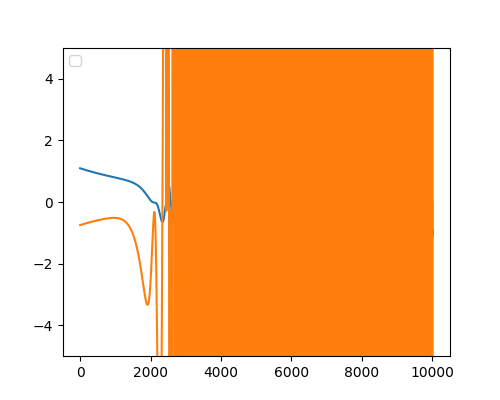
\includegraphics{Plots.png}
\begin{center}
Function plot is blue, Derivative plot is orange, MacLoren series plot is green
\end{center}
\end{document}